% !TeX root = ../../main.tex
\documentclass[../AAE590LGM_HW3.tex]{subfiles}
\begin{document}

\subsection{1.b) \textbf{Bank-to-Turn, Trajectory, and Simulation:}}
% Turning radius plot
\begin{figure}[H]
    \caption{Turning radius plot}
    \centering
    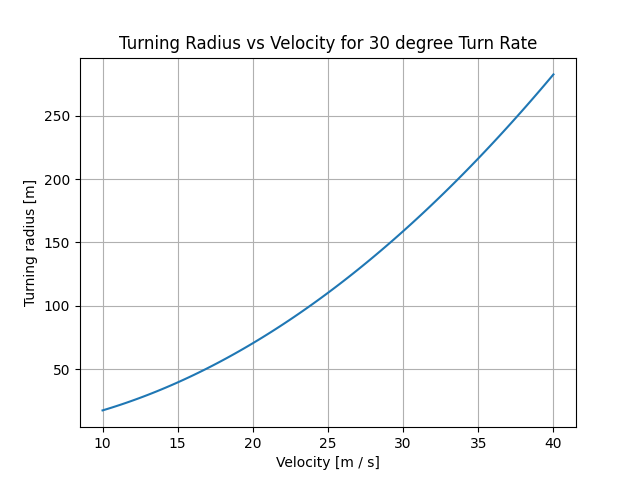
\includegraphics[width=0.7\linewidth]{AAE590LGM_HW3_Q1_turn_radius.png}
\end{figure}

% Reference trajectory plot
\begin{figure}[H]
    \caption{Reference trajectory plot}
    \centering
    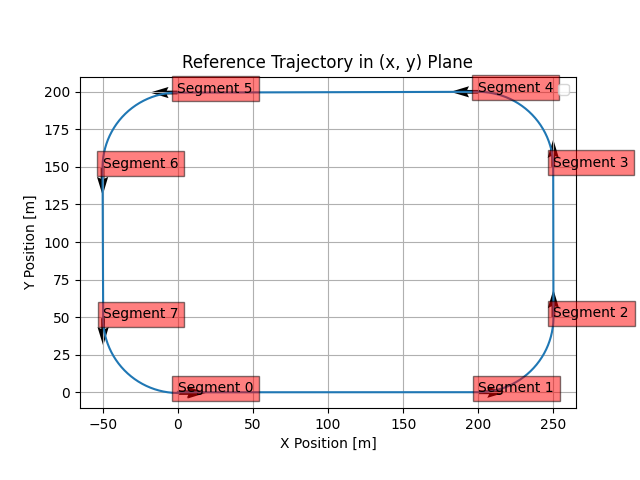
\includegraphics[width=0.7\linewidth]{AAE590LGM_HW3_Q1_reftraj.png}
\end{figure}

% Feasibility check (phi < 45 deg)
\begin{figure}[H]
    \caption{Feasibility check of turn required bank angles}
    \centering
    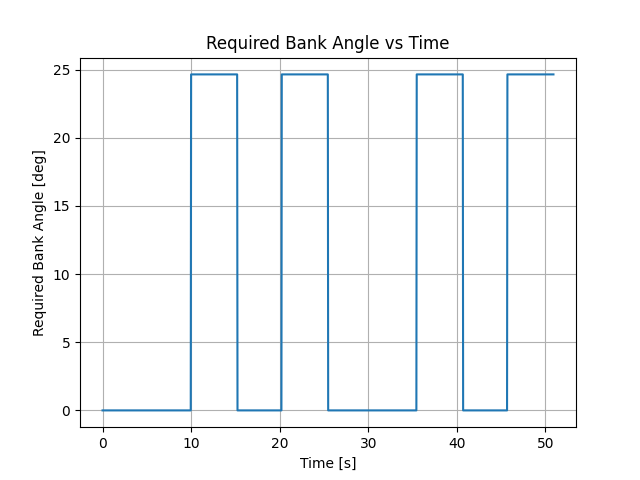
\includegraphics[width=0.7\linewidth]{AAE590LGM_HW3_Q1_feasck.png}
\end{figure}

% Simulate linus and loopy
\begin{figure}[H]
    \caption{Plots of Linus and Loopy simulation}
    \centering
    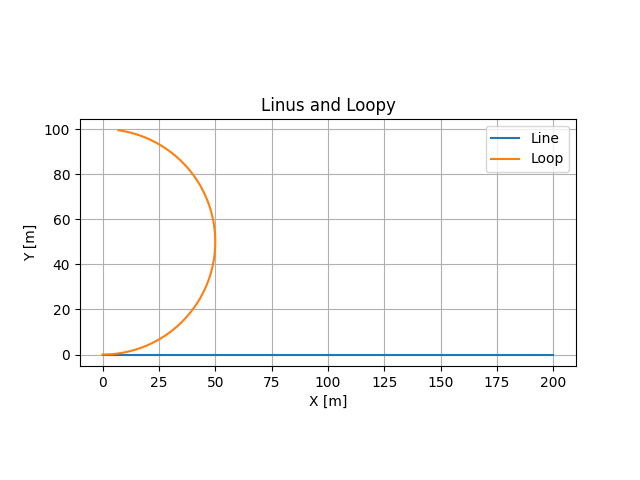
\includegraphics[width=0.7\linewidth]{AAE590LGM_HW3_Q1_linusloopy.png}
\end{figure}

% Code
\lstinputlisting[language=Python,caption={SE(2) Fixed-Wing Velocity Kinematics Code}]{AAE590LGM_HW3_Q1.py}


\end{document}
